\documentclass[serif, aspectratio=169]{beamer}
\usepackage[T1]{fontenc} 
\usepackage{fourier}
\usepackage{hyperref}
\usepackage{latexsym,amsmath,xcolor,multicol,booktabs,calligra}
\usepackage{booktabs} % For better table formatting
\usepackage{graphicx,pstricks,listings,stackengine}
\usepackage{listings}
\usepackage{array} 
\usepackage{colortbl}

\author{Dr.Hajialiasgari}
\title{Machine Learning}
\institute{
    Tehran University \\
    Of\\
    Medical Science
}
\date{\small \today}
\usepackage{UoWstyle}

% Define custom colors and styles for listings
\definecolor{deepblue}{rgb}{0,0,0.5}
\definecolor{deepred}{RGB}{153,0,0}
\definecolor{deepgreen}{rgb}{0,0.5,0}
\definecolor{halfgray}{gray}{0.55}

\lstset{
    basicstyle=\ttfamily\small,
    keywordstyle=\bfseries\color{deepblue},
    emphstyle=\ttfamily\color{deepred},
    stringstyle=\color{deepgreen},
    numbers=left,
    numberstyle=\small\color{halfgray},
    rulesepcolor=\color{red!20!green!20!blue!20},
    frame=shadowbox,
}

\begin{document}

\begin{frame}
    \titlepage
    \vspace*{-0.6cm}
    \begin{figure}[htpb]
        \begin{center}
            \includegraphics[keepaspectratio, scale=0.05]{Tumsl-logo.png}
        \end{center}
    \end{figure}
\end{frame}

\begin{frame}    
\tableofcontents[sectionstyle=show, subsectionstyle=show/shaded/hide, subsubsectionstyle=show/shaded/hide]
\end{frame}

\section{Introduction}
\begin{frame}{What is Classification?}
\textbf{Classification} is a supervised learning task where the goal is to predict the category or class label of a given input based on its features. It involves learning a decision boundary that separates different classes in the data.
\end{frame}

\begin{frame}{Binary Classification Examples}
\begin{itemize}
    \item \textbf{Medical Diagnosis:} Predicting whether a tumor is \textit{benign} or \textit{malignant}.
    \item \textbf{Spam Detection:} Classifying emails as \textit{spam} or \textit{not spam}.
    \item \textbf{Loan Approval:} Predicting whether a loan application is \textit{approved} or \textit{rejected}.
    \item \textbf{Weather Prediction:} Classifying if it will \textit{rain} or \textit{not rain} tomorrow.
\end{itemize}
\end{frame}

\begin{frame}{Classification Problem}
\textit{Can we solve this problem by Linear Regression?}
\begin{minipage}{0.48\linewidth}
        \centering
        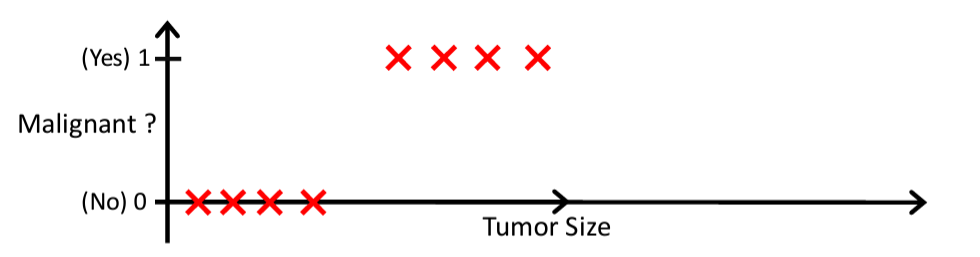
\includegraphics[width=\linewidth]{Classification1png.png}
    \end{minipage}
    \hfill
    \begin{minipage}{0.48\linewidth}
        \centering
        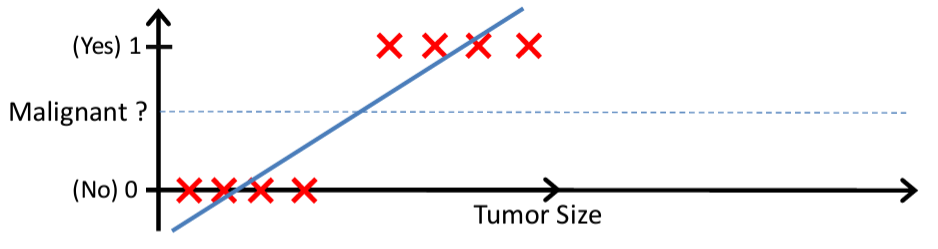
\includegraphics[width=\linewidth]{Classification2.png}
    \end{minipage}
\vspace{0.5cm}
\textit{We could fit a straight line and define a threshold at 0.5:}
\begin{itemize}
    \item If $h_\theta(x) \geq 0.5$, predict $y = 1$
    \item If $h_\theta(x) < 0.5$, predict $y = 0$
\end{itemize}
\end{frame}

% Slide: What about now?
\begin{frame}{Classification Problem}
    \begin{itemize}
        \item What about now? (By adding a new data point)
    \end{itemize}

    \centering
    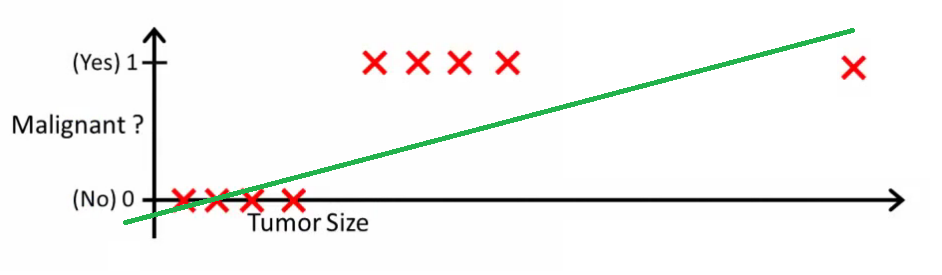
\includegraphics[width=\linewidth]{linear-regression-classification.png}
    

\begin{itemize}
    \item \textbf{Classification:} $y = 0$ or $y = 1$
    \item $h_\theta(x)$ can be $> 1$ or $< 0$
    \item Another drawback of using linear regression for this problem
\end{itemize}

\vspace{0.5cm}
\textbf{What we need:}
\begin{itemize}
    \item Logistic regression: $0 \leq h_\theta(x) \leq 1$
    \item We also show this function with other notations: $f(x; w) = \sigma(w^T x)$
\end{itemize}
\end{frame}

\section{Logistic Regression}

\begin{frame}{Introduction}
\textbf{Problem:} Distinguish if a person is \textit{overweight} or \textit{not overweight} based on features like age, gender, height, weight, and BMI.

\begin{table}[h]
\centering
\begin{tabular}{|c|c|c|c|c|c|}
\hline
Age & Gender & Height (cm) & Weight (kg) & BMI & Overweight \\
\hline
25 & Male & 175 & 80 & 25.3 & 0 \\
30 & Female & 160 & 60 & 22.5 & 0 \\
... & ... & ... & ... & ... & ... \\
35 & Male & 180 & 90 & 27.3 & 1 \\
\hline
\end{tabular}
\end{table}

\vspace{0.5cm}
\textbf{Notation:}
\begin{itemize}
    \item Features of a sample: \textbf{vector} $x$
    \item Label: $y$
\end{itemize}

\vspace{0.5cm}
\textbf{Logistic Regression:} We try to find a function $\sigma(w^T x)$ that predicts the posterior probabilities $P(y = 1 \mid x)$.
\end{frame}

\begin{frame}{Introduction (cont.)}
    \begin{itemize}
        \item $\sigma (w^Tx)$: probability that $y=1$ given $x$ (parameterized by \textbf{$\textbf{w}$})
      \begin{align*}
        P(y=1|x,\mathbf{w}) &= \sigma (\mathbf{w}^Tx) \\
        P(y=0|x,\mathbf{w}) &= 1 - \sigma (\mathbf{w}^Tx)
      \end{align*}

        \item We need to look for a function which gives us an output in the range [0, 1]. (like a probability).

        \item Let's denote this function with $\sigma (.)$ and call it the \textbf{activation function}.
        
    \end{itemize}
\end{frame}

\begin{frame}{Introduction (cont.)}
    \begin{minipage}{0.55\textwidth}
    \begin{itemize}
        \item Sigmoid (logistic) function.
        \[
            \sigma (z) = \frac{1}{1 + e^{-z}}
        \]
        \item A good candidate for activation function.
        
        \item It gives us a number between 0 and 1 \textbf{smoothly}.
        \item It is also \textbf{differentiable}

    \end{itemize}
    \end{minipage}% 
    \begin{minipage}{0.4\textwidth}
        \centering
        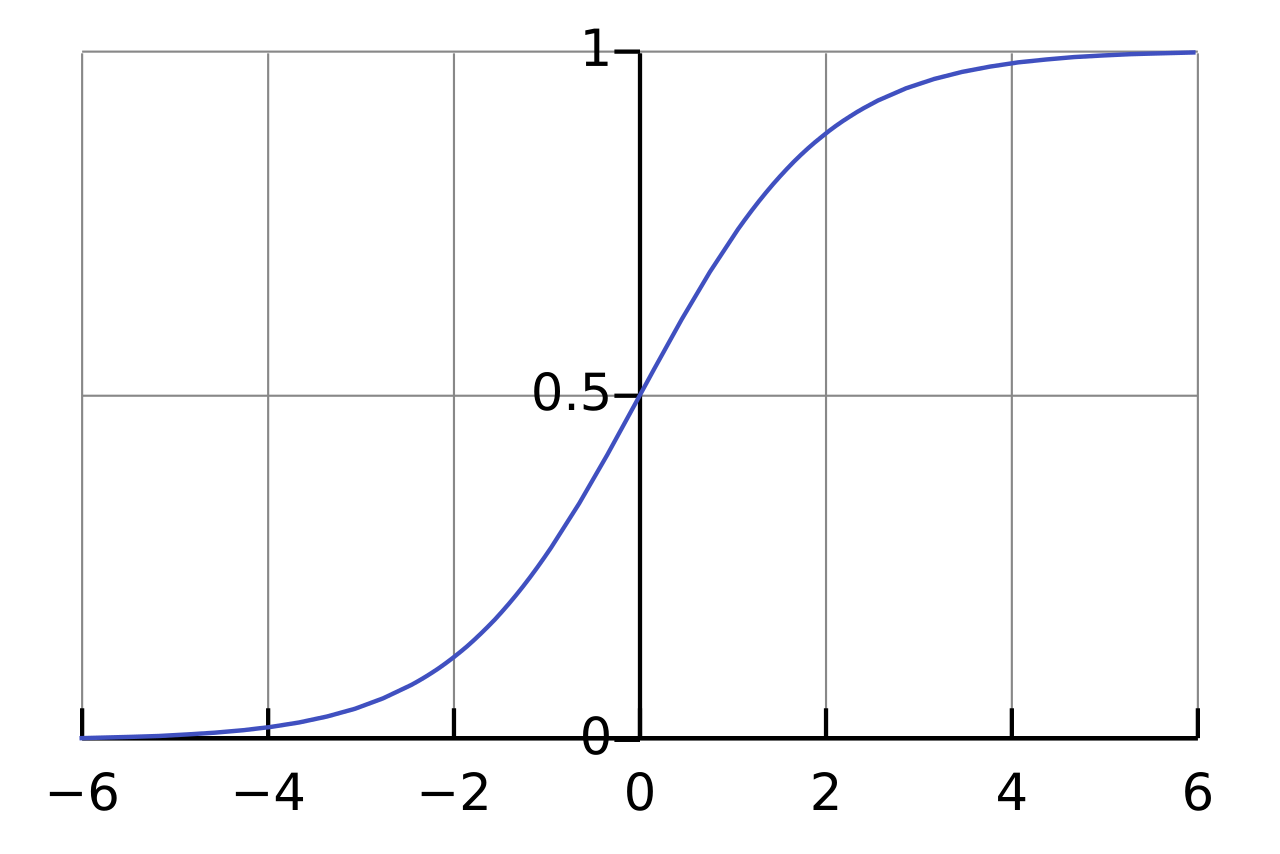
\includegraphics[width=0.8\textwidth]{Logistic-curve.svg.png}
    \end{minipage}
\end{frame}

\begin{frame}{Sigmoid function \& its derivative}
    \centering
        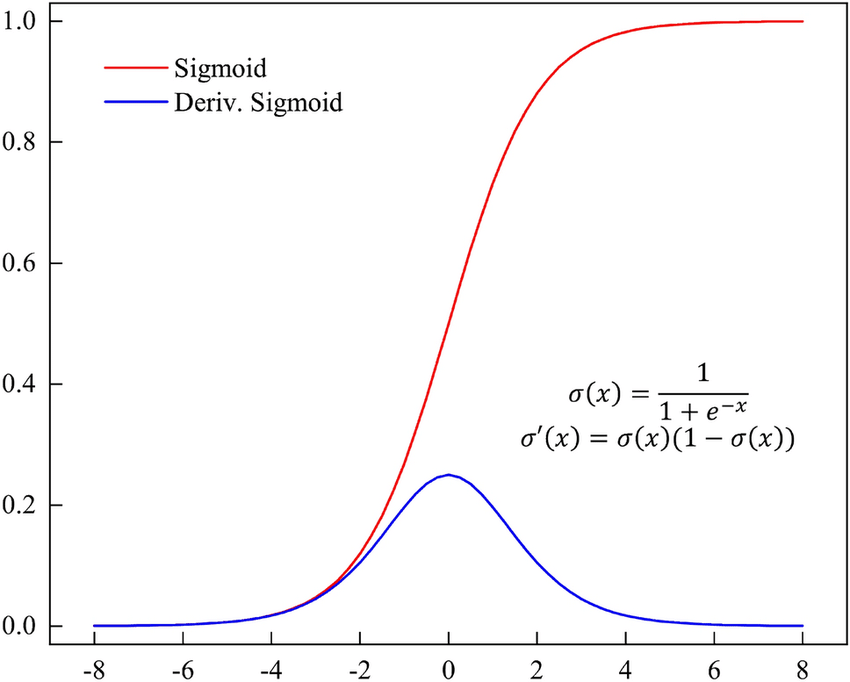
\includegraphics[width=0.5\textwidth]{Sigmoid-Derivative.png}
\end{frame}

\begin{frame}{Introduction (cont.)}
    \begin{itemize}
      \item The sigmoid function takes a number as input but we have:
    \end{itemize}
        \begin{align*}
            x &= [x_0=1,x_1, \dots, x_d] \\
            w &= [w_0, w_1, \dots, w_d]
        \end{align*}
    \begin{itemize} 
      \item So we can use the \textbf{dot product} of $x$ and $w$.
      
      \item We have $0\leq \sigma (\mathbf{w}^Tx) \leq 1$. which is the estimated probability of $y=1$ on input $x$.

      \item An Example : A basketball game (Win, Lose)
        \begin{itemize}
            \item $\sigma (\mathbf{w}^T x) = 0.7$
            \item In other terms $70$ percent chance of winning the game.
        \end{itemize}
        
    \end{itemize}
\end{frame}

\begin{frame}{Decision surface}
    \begin{itemize}
      \item Decision surface or decision boundary is the region of a problem space in which the output label of a classifier is ambiguous. (could be linear or non-linear)
      \item In binary classification it is where the probability of a sample belonging to each $y=0$ and $y=1$ is equal.
    \end{itemize}
    
     \begin{center}
        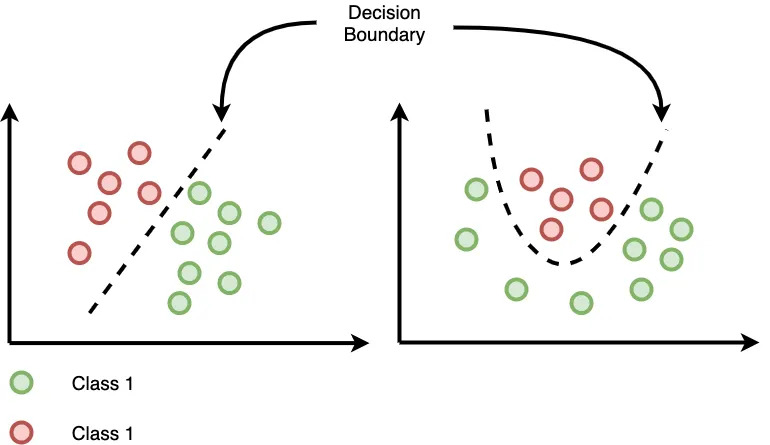
\includegraphics[width=0.4\textwidth]{decision-boundry.jpg}
    \end{center}
    
    \begin{itemize}
      \item Decision boundary hyperplane always has \textbf{one less dimension} than the feature space.
     
    \end{itemize}
\end{frame}

\begin{frame}{Decision surface (cont.)}
    \begin{itemize}
        \item An example of linear decision boundaries:
    \end{itemize}
    \begin{center}
        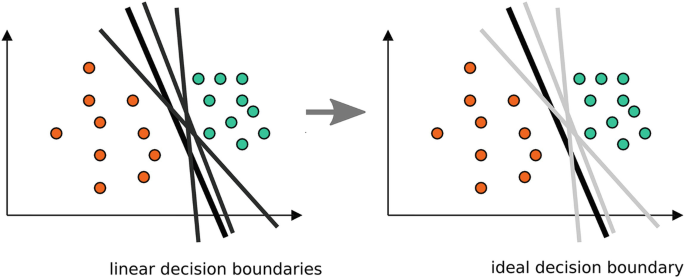
\includegraphics[width=0.85\textwidth]{decision-boundry1.png}
    \end{center}
\end{frame}

\begin{frame}{Decision surface (cont.)}
    \begin{itemize}
      \item Back to our logistic regression problem.
      \item Decision surface $\sigma (\mathbf{w}^Tx) = $ \textbf{constant}.
        \[
            \sigma (\mathbf{w}^Tx) = \frac{1}{1 + e^{-(\mathbf{w}^Tx)}} = 0.5
        \]
      \item Decision surfaces are \textbf{linear functions} of $x$
        \begin{itemize}
            \item if $\sigma (\mathbf{w}^Tx) \geq 0.5$ then $\hat{y}=1$, else $\hat{y} = 0$
            \item Equivalently, if $\mathbf{w}^Tx + w_0 \geq 0.5$ then decide $\hat{y}=1$, else $\hat{y}=0$
        \end{itemize}% ayoub eshgh
        \vfill
        \begin{center}
            \( \hat{y} \) \textbf{is the predicted label}
        \end{center}
    \end{itemize}
\end{frame}

\begin{frame}{Non-Linear Boundary Example}
    \centering
    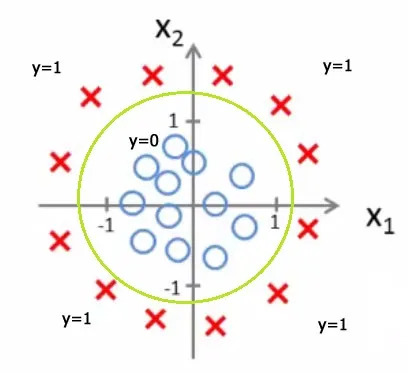
\includegraphics[width=0.45\textwidth]{non-linear-boundry.jpg}
    
    \begin{align*}
        \text{Predict } y=1 \text{ if } -1 + x_12 + x_22 \geq 0 \end{align*}
\end{frame}

\section{Evaluation}

\begin{frame}{Quote of the Day}
\centering
\textit{“It doesn't matter how beautiful your theory is ... If it doesn't agree with experiment, it's wrong.”} \\[0.5cm]
― Richard Feynman
\end{frame}


\begin{frame}{Confusion Matrix and Accuracy}
\textbf{Confusion Matrix:}
\begin{table}[]
\centering
\begin{tabular}{|c|c|c|}
\hline
                & \textbf{Predicted Positive} & \textbf{Predicted Negative} \\\hline
\textbf{Actual Positive} & True Positive (TP) & False Negative (FN) \\\hline
\textbf{Actual Negative} & False Positive (FP) & True Negative (TN) \\\hline
\end{tabular}
\end{table}

\textbf{Accuracy:}
\[
\text{Accuracy} = \frac{TP + TN}{TP + TN + FP + FN}
\]
\end{frame}
\begin{frame}{Example: Cancer Detection}
\begin{itemize}
    \item \textbf{Scenario:} Predicting whether a tumor is malignant (1) or benign (0).
    \item \textbf{Confusion Matrix:}
\end{itemize}
\begin{table}[]
\centering
\begin{tabular}{|c|c|c|}
\hline
                & \textbf{Predicted Malignant} & \textbf{Predicted Benign} \\\hline
\textbf{Actual Malignant} & 50 (TP) & 10 (FN) \\\hline
\textbf{Actual Benign} & 5 (FP) & 85 (TN) \\\hline
\end{tabular}
\end{table}

\textbf{Calculations:}
\begin{itemize}
    \item \textbf{Accuracy:} $\frac{50 + 85}{50 + 85 + 10 + 5} = 0.935$ (93.5\%).
    \item \textbf{Precision:} $\frac{50}{50 + 5} = 0.909$ (90.9\%).
    \item \textbf{Recall:} $\frac{50}{50 + 10} = 0.833$ (83.3\%).
\end{itemize}
\end{frame}

% Slide 2: Precision and Recall
\begin{frame}{Precision and Recall}
\textbf{Precision:}
\[
\text{Precision} = \frac{TP}{TP + FP}
\]
\textit{Focus: How many positive predictions are actually correct.}

\textbf{Recall (Sensitivity):}
\[
\text{Recall} = \frac{TP}{TP + FN}
\]
\textit{Focus: How many actual positives are correctly identified.}
\end{frame}

% Slide 3: F1 Score
\begin{frame}{F1 Score}
\textbf{F1 Score:}
\[
F1 = 2 \cdot \frac{\text{Precision} \cdot \text{Recall}}{\text{Precision} + \text{Recall}}
\]
\textit{Use: Balances Precision and Recall, especially in imbalanced datasets.}
\end{frame}

% Slide 4: ROC Curve and AUC
\begin{frame}{ROC Curve and AUC}
\textbf{ROC Curve:}
\begin{itemize}
    \item Plots True Positive Rate (TPR) vs. False Positive Rate (FPR).
    \item Evaluates classifier performance at various thresholds.
\end{itemize}

\textbf{AUC:}
\begin{itemize}
    \item Measures the overall ability of the model to distinguish between classes.
    \item Range: 0.5 (No discrimination) to 1.0 (Perfect discrimination).
\end{itemize}
\end{frame}

\begin{frame}{ROC-AUC}
    \centering
    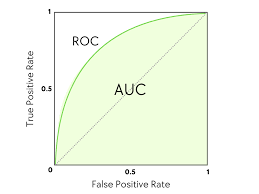
\includegraphics[width=0.45\textwidth]{ROC-AUC.png}
\end{frame}

% Slide 5: Log-Loss
\begin{frame}{Log-Loss (Logarithmic Loss)}
\textbf{Formula:}
\[
\text{Log-Loss} = -\frac{1}{n} \sum_{i=1}^n \Big[y^{(i)} \log(p^{(i)}) + (1 - y^{(i)}) \log(1 - p^{(i)})\Big]
\]
\textit{Use: Penalizes incorrect predictions with confidence.}
\end{frame}

% Slide 6: Specificity
\begin{frame}{Specificity (True Negative Rate)}
\textbf{Formula:}
\[
\text{Specificity} = \frac{TN}{TN + FP}
\]
\textit{Focus: How many negatives are correctly identified.}
\end{frame}

% Slide 7: Summary of Evaluation Metrics
\begin{frame}{Summary of Evaluation Metrics}
\begin{table}[]
\centering
\begin{tabular}{|c|c|c|}
\hline
\textbf{Metric} & \textbf{Formula} & \textbf{Use Case} \\\hline
Accuracy & \(\frac{TP + TN}{TP + TN + FP + FN}\) & Overall correctness \\\hline
Precision & \(\frac{TP}{TP + FP}\) & Positive prediction quality \\\hline
Recall & \(\frac{TP}{TP + FN}\) & Positive detection rate \\\hline
F1 Score & \(2 \cdot \frac{\text{Precision} \cdot \text{Recall}}{\text{Precision} + \text{Recall}}\) & Balancing Precision and Recall \\\hline
Specificity & \(\frac{TN}{TN + FP}\) & Negative detection rate \\\hline
Log-Loss & $-\frac{1}{n} \sum \log$ & Probabilistic predictions \\\hline
\end{tabular}
\end{table}
\end{frame}



\begin{frame}
    \begin{center}
        {\Huge\ \color{red}For more information and code check the related notebook}
    \end{center}
\end{frame}


\begin{frame}
    \begin{center}
        {\Huge\ End of Classification}
    \end{center}
\end{frame}

\end{document}

